% Template for Cogsci submission with R Markdown

% Stuff changed from original Markdown PLOS Template
\documentclass[10pt, letterpaper]{article}

\usepackage{cogsci}
\usepackage{pslatex}
\usepackage{float}
\usepackage{caption}

% amsmath package, useful for mathematical formulas
\usepackage{amsmath}

% amssymb package, useful for mathematical symbols
\usepackage{amssymb}

% hyperref package, useful for hyperlinks
\usepackage{hyperref}

% graphicx package, useful for including eps and pdf graphics
% include graphics with the command \includegraphics
\usepackage{graphicx}

% Sweave(-like)
\usepackage{fancyvrb}
\DefineVerbatimEnvironment{Sinput}{Verbatim}{fontshape=sl}
\DefineVerbatimEnvironment{Soutput}{Verbatim}{}
\DefineVerbatimEnvironment{Scode}{Verbatim}{fontshape=sl}
\newenvironment{Schunk}{}{}
\DefineVerbatimEnvironment{Code}{Verbatim}{}
\DefineVerbatimEnvironment{CodeInput}{Verbatim}{fontshape=sl}
\DefineVerbatimEnvironment{CodeOutput}{Verbatim}{}
\newenvironment{CodeChunk}{}{}

% cite package, to clean up citations in the main text. Do not remove.
\usepackage{apacite}

% KM added 1/4/18 to allow control of blind submission


\usepackage{color}

% Use doublespacing - comment out for single spacing
%\usepackage{setspace}
%\doublespacing


% % Text layout
% \topmargin 0.0cm
% \oddsidemargin 0.5cm
% \evensidemargin 0.5cm
% \textwidth 16cm
% \textheight 21cm

\title{Discovering Conceptual Structure Through Explicit and Implicit Cues in
Child-Directed Speech}

\usepackage{dcolumn}

\author{{\large \bf Anonymous CogSci submission}}

\begin{document}

\maketitle

\begin{abstract}
In order for children to understand and reason about the world in a
mature fashion, they need to learn that conceptual categories are
organized in a hierachical fashion (e.g., a dog is also an animal). The
caregiver lingusitic input can play an important role in this learing,
and previous studies have documented several cues in parental talk that
can help children learn a conceptual hierachy. However, these previous
studies used different datasets and methods which made difficult the
systematic comparison of these cues and the study of their relative
contribution. Here, we use a large-scale coprus of child-directed speech
and a classificatin-based evaluation method which allowed us to
investigate, within the same framework, various cues that varied
radically in terms of how explicit the information they offer is. We
found the most explcit cues to be too sparse or too noisy to support
robust learning (though part of the noise may be due to imperfect
operationalization). In contrast, the implicit cues offered, overall, a
reliable source of information. Our work confirms the utility of
caregiver talk for conveying conceptual information. It provides a
stepping stone towards a cognitive model that would use this information
in a principled way, possibly leading to testable predictions about
children's conceptual development

\textbf{Keywords:}
Conceptual learning, child-directed speech, language and cognition
\end{abstract}

\hypertarget{introduction}{%
\section{Introduction}\label{introduction}}

A hallmark of conceptual knowledge is its hierarchical organization. For
example, a husky can be categorized as a dog, but it can also be
categorized as a mammal, an animal, or a living being. Hierarchical
organization is fundamental to human cognition as it allows, among other
things, the generalization of knowledge through inference. For example,
upon learning that all living beings are made out of cells, one can
conclude that dogs are made of cells, too.

How do children acquire conceptual hierarchy? Early accounts considered
conceptual hierarchy to be the consequence of the emergence of a
domain-general logic of class-inclusion -- in other words grasping the
idea that one category can be part of a larger one (Inhelder \& Piaget,
2013; Sloutsky, 2015). Children can acquire hierarchy in a specific
domain before mastering the domain-general logic of classes, however
(Carey, 1987; Chi, Hutchinson, \& Robin, 1989; Inagaki \& Hatano, 2002;
Keil, 1981), suggesting that category-specific input may play a role in
this development.

There are signs that children as young as 3 years old show hierarchical
knowledge in various domains (e.g., animals, clothes, and food). Such
signs include using superordinate words like ``food'' and ``animal''
according to parental report (Fenson et al., 1994), using different
words to label the same object at different levels of conceptual
hierarchy (Clark, 1997), and being able to extend the meaning of novel
words to superordinate categories even controlling for perceptual
similarity (Liu, Golinkoff, \& Sak, 2001).

Do children learn conceptual hierarchy from the language that they hear?
Analyses of parent-child interactions have shown that parents rarely
introduce words at the superordinate-level without also providing the
basic level term (Blewitt, 1983; Callanan, 1985; Shipley, Kuhn, \&
Madden, 1983). For example, parents rarely point to an object and say
``this is an animal!''. Instead, they usually anchor the superordinate
word ``animal'' at the basic level by saying something along the lines
of ``This is a duck; a duck is a kind of animal.'' Such an anchoring
strategy provides children with a categorization of the same object at
different levels, which may help children understand the underlying
hierarchical organization.

In a different line of research prompted by recent advances in data
science (Landauer \& Dumais, 1997; Mikolov, Sutskever, Chen, Corrado, \&
Dean, 2013), researchers have found that the statistical distribution of
basic-level terms in parental speech can lead to a coherent structures
at the superordinate level (Fourtassi, Scheinfeld, \& Frank, 2019;
Huebner \& Willits, 2018). To illustrate, one can learn that ``horse''
and ``dog'' are part of a higher-level category just by observing that
these words co-occur in similar contexts. This distributional
co-occurrence cue can be a powerful source of conceptual hierarchy
because it is based on pure co-occurrence and does not require the
presence of a lexicalized label for the higher-level category. On this
kind of account, categories emerge in a bottom-up fashion as a cluster
of related words at the lower-level.

Both these cues -- explicit anchoring and implicit distributional
co-occurrence learning -- could in principle be helpful for children. In
the case of the ``is-a-kind-of'' anchoring, there is evidence that
preschool children ably use this cue to interpret the meaning of a novel
word at the superordinate level (Callanan, 1989). In the case of pure
co-occurrence, extensive research in the last couple of decades has
shown that children are capable of tracking distributional statistics of
various linguistic units (Saffran, Aslin, \& Newport, 1996). Further,
children appear to rely on the way words co-occur in speech to make
conceptual generalizations (Fisher, Matlen, \& Godwin, 2011; Matlen,
Fisher, \& Godwin, 2015).

The cues reviewed above can be thought of as ends in a continuum that
varies from explicit to implicit. The ``is-a-kind-of'' cue is the most
explicit cue since both the terms (i.e., the basic and superordinate
labels) and their hierarchical relationship are explicitly stated. The
pure co-occurrence cue is the most implicit cue since, on the one hand,
the superordinate term is not required and, on the other hand, the
hierarchical relationship (that is, the fact that co-occurring basic
level terms are part of a higher-level category) can only be induced.

While previous studies have focused on these extremes, other cues are
available that have an intermediate status on this continuum. Here, we
examine the way parents hint at the hierarchical relationship between
two concepts pragmatically without using an explicit inclusion
expression. For example, instead of saying ``a cow is a kind of animal''
parents can say the following (e.g., in the context of a play session):
``Do you want a cow or do you want another animal?'' (see Table 1 for
more examples). We also study whether action affordances provide another
-- perhaps more explicit, but still distributional -- cue for category
membership. For example, food items could be identified as members of a
category by virtue of their compatibility with the verb ``eat'' and
clothing items by their compatibility with ``wear.''

Previous studies examining individual cues to categorization vary in
terms of both the datasets and methods they have used, which makes
comparison difficult. Implicit cues have generally been studied using
large-scale data and have been evaluated based on their ability to
provide an accurate similarity space for words. In contrast, explicit
cues have been studied mainly in the context of small-scale experiments
and have been tested mainly through counting the frequency of a given
linguistic expression (e.g., ``X is a kind of Y'').

In this work, we make a systematic comparison of explicit and implicit
cues using similar methods. Such comparison is crucial as it allows us,
for instance, to quantify the relative role that each cue could play in
development. More precisely, we take a classification approach: We
operationalize different cues as features that can be used to compute
similarity. We then evaluate this continuous similarity measure by using
it for a classification task, deciding whether different basic-level
categories are part of the same superordinate category. Thus we can
assign a classification accuracy to each cue type. We begin by
introducing our dataset and the set of conceptual cues we consider; we
then present results from this classification task.

\begin{CodeChunk}
\begin{figure*}[h]

{\centering 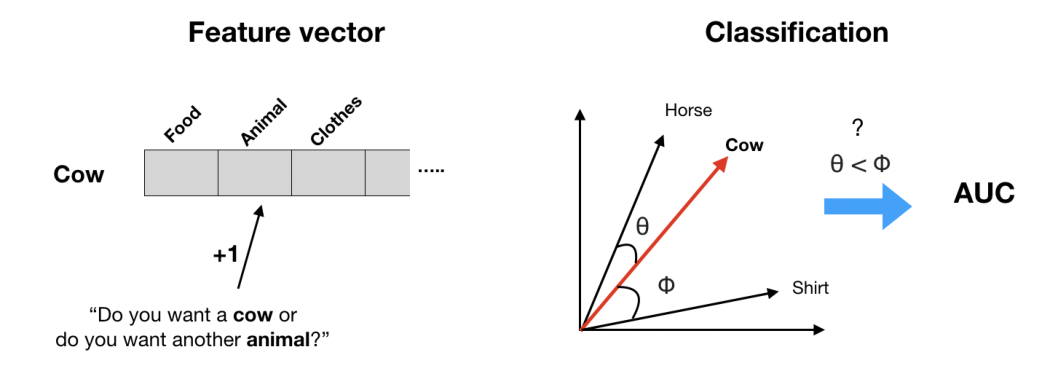
\includegraphics{cogsci_files/figure-latex/task-1} 

}

\caption{\label{fig:task} A schematic description of the task. For each basic-level word (here, 'cow') a feature vector is derived from child-directed speech based on how the cue is defined. Here, the vector cells correspond to the superordinate categories. The entry in a given cell (e.g., animal) is incremented when the word 'cow' co-occurs with the corresponding category label. The cue is evaluated based on its ability to classify pairs of words into 'same' or 'different' superordinate categories. Here, the pair 'cow'-'horse' belongs to the same category. The corresponding vectors should be closer to each other than the vectors of a pair that belongs to different categories (e.g., 'cow'-'shirt'). This evaluation is quantified by a standard measure in signal detection theory called the Area Under the ROC Curve (AUC).}\label{fig:task}
\end{figure*}
\end{CodeChunk}

\hypertarget{analyses}{%
\section{Analyses}\label{analyses}}

\hypertarget{data}{%
\subsection{Data}\label{data}}

We constructed a large-scale corpus by aggregating over all
English-language transcripts from CHILDES (MacWhinney, 2014; Sanchez et
al., 2019). These transcripts involved the caregivers' speech addressed
to children up to three years of age. We had a total of XXX transcripts,
across XXXX unique children, yielding a total of XXX utterances.

We decided to study the six following superordinate categories:
``animal'', ``furniture'', ``clothes'', ``food'', ``toys'' and
``vehicles''. For each of these categories, we used the corresponding
basic-level terms available in the English-language MacArthur-Bates
Communicative Inventory (CDI) (Fenson et al., 1994), a parent-report
instrument that provide a partial listing and categorization of words
produced by children 18--30 months. These categories were chosen because
they were the optimal set of superordinate categories that had been
studied previously and CDI data were available. Most previous
experimental work (which we parlty reviewed above) used only a subset of
these categories for a given study.

\hypertarget{cues-to-conceptual-hierarchy-and-their-feature-vectors}{%
\subsection{Cues to Conceptual Hierarchy and their Feature
Vectors}\label{cues-to-conceptual-hierarchy-and-their-feature-vectors}}

As indicated above, we explored four cues to conceptual hierarchy:
``is-a-kind-of'', pragmatic, verb affordance-based, and pure
co-occurrence cues. We represented each cue as a set of features and we
tested how these features allow us to classify basic-level terms into
superordinate categories. To this end, we started by using each cue to
derive a feature vector for each basic-level word in the CDI lexicon. In
the case where the cue relied on an explicit category marker (i.e., the
first three cues), the feature vectors were based on the superordinate
categories introduced above. Otherwise (e.g., the fourth cue), the
feature vector was an embedding in a high dimensional space derived
based on the words' pattern of co-occurrence only. In the following, we
explain how we computed the feature vectors for each cue (see also
Figure \ref{fig:task}).

\hypertarget{is-a-kind-of}{%
\subsubsection{Is-a-kind-of}\label{is-a-kind-of}}

This cue tests the extent to which parents use explicit expressions of
class inclusion (Callanan, 1985). For each word at the basic label, X,
we construct a feature vector of length 6, where every cell corresponds
to a superordinate category, Y, and the entry in each cell corresponds
to the frequency with which X appears with Y is in one of the following
expressions: ``X is a/an Y'' and ``X is a kind of Y'' (we kept the same
expressions used in previous studies).

\begin{table}[!htbp] \centering 
\begin{tabular}{l p{.35\textwidth}}
\hline

\textbf{Animals} & Do you want a cow or do you want another animal?\\

\textbf{Furniture} & Furniture means sofa and chair and...\\

\textbf{Clothes} & This is another clothes. See, it's just like this shirt.\\

\textbf{Food}   & She asks Lily what her favorite food is. If Lily says chocolate I am in trouble. \\

\textbf{Toys} & You close the book and get another toy because I think we are tired of this.\\

\textbf{Vehicles} & The only vehicle you cut out so far is the train.\\

\hline
\end{tabular}
\caption{\label{tab:pragmatic} Examples of utterances from CHILDES where parents hint at a hierachical relations between basic- and superordinate- level terms.}
\end{table}

\hypertarget{pragmatic}{%
\subsubsection{Pragmatic}\label{pragmatic}}

Parents can express conceptual hierarchy between X and Y without
necessarily using an ``is-a-kind-of'' expression. In many cases, parents
can hint at this hierarchy using a wide diversity of linguistic
expressions (Table 1). Detecting these expressions at scale is a
challenge given their complexity, so as a first attempt to capture this
diversity, we relax grammatical constraints between X to Y, and we keep
only the requirement that X and Y should co-occur.

More concretely, we represent each basic-level term, X, with a feature
vector where each entry represents the frequency with which X co-occurs
with the corresponding superordinate term Y. This co-occurrence is
determined using a fixed window of \(k\) utterances. Values of \(k > 1\)
allow us to capture the case where a relationship between X and Y is
established across more than one utterance. For example:

-- Mother : What kind of animal is this?

-- Mother : It's a giraffe!

\hypertarget{affordance-based}{%
\subsubsection{Affordance-based}\label{affordance-based}}

The super-ordinate label is not the only category marker that can cue
conceptual hierarchy for a basic level term, especially when this
category can be characterized by an affordance. For example, ``food''
can be characterized as the category of things we eat and ``clothes'' as
things we wear. Thus, children can learn that some concepts (e.g.,
``apple'' and ``bread'') are parts of a higher-level category (``things
we eat'') by observing how these concepts co-vary with a cue of their
common affordance (i.e., the verb ``eat'').

We computed the feature vectors for this cue as follows. In a first
step, we tried to find a single verb that could be used as an affordance
marker for an entire category. We used ``eat'' for food, ``wear'' for
clothes, ``play'' for toys, and ``ride'' for vehicles. The category
``furniture'' has no such obvious function verb. We decided to use the
verb ``use'' because if there were a verb that could fit every member of
the category of furniture, it would be that (even though it can also fit
things that are not members of the category). For the animal category,
we could find no verb that could categorize the instances.

We detected the concept-affordance relationship, syntactically, based on
their occurrence in a verb-complement
structure.\footnote{There are more complex structures that could, in principle, be used by parents. We used the simplest as a first approximation, though the performance of this cue could likely be enhanced by considering a wider variety of constructions.}
For example, in the utterance ``the bird eats the berries'', the word
``berries'' was categorized as ``eat''-able. For each basic-level term,
we computed a feature vector where entries correspond to the frequency
with which this term occurs in a verb-complement relationship with the
verb/affordance at hand.

\hypertarget{pure-co-occurrence}{%
\subsubsection{Pure Co-occurrence}\label{pure-co-occurrence}}

Unlike the first three cues, the pure co-occurrence cue is not based on
an explicit category marker at the superordinate level. It is based,
instead, on the way basic-level terms are distributed together in speech
(Harris, 1957). Following previous research (Fourtassi et al., 2019), we
quantified this cue using the word embedding model Word2Vec (Mikolov et
al., 2013). We used this model to represent basic-level words as vectors
in a high-dimensional space, representing the distribution of these
words in a latent semantic structure.

\hypertarget{task-and-evaluation}{%
\subsection{Task and Evaluation}\label{task-and-evaluation}}

Above, we characterized all cues in a vectorial framework. This
framework allows us to directly compare the cues in terms of how they
quantify the similarity between words (defined as the cosine of the
angle formed by their vectors). Based on this similarity, we test the
ability of each cue to predict which pairs of words belong to the same
superordinate category (e.g., ``apple'' and ``bread'') and which pairs
of words belong to different categories (e.g., ``apple'', ``horse'')
(Figure \ref{fig:task}).

\begin{CodeChunk}
\begin{figure*}[h]

{\centering 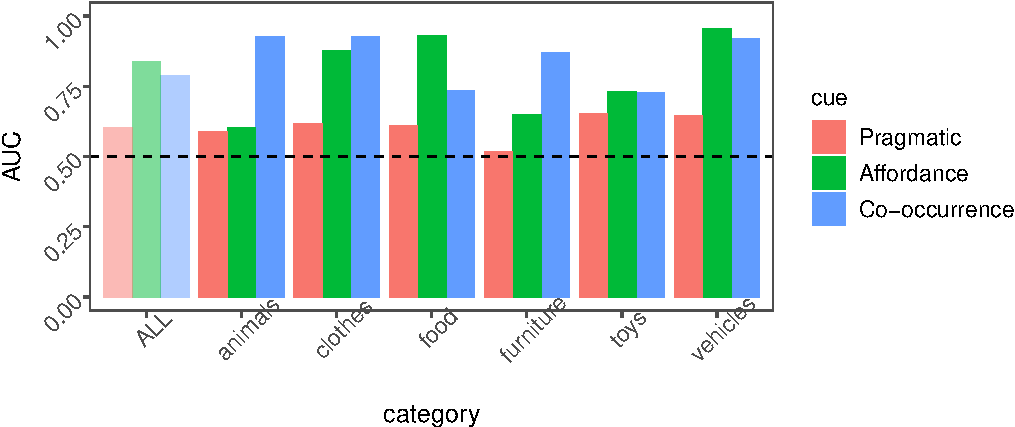
\includegraphics{cogsci_files/figure-latex/all_data-1} 

}

\caption{\label{fig:data_all} The Area Under the ROC Curve (AUC) scores for each cue across all categories ('ALL') and for each category. A value of 0.5 represents pure chance, and a value of 1 represents perfect performance. The AUC score can be interpreted as the probability that, given two pairs of basic-level words, of which one is from the same superordinate category, the pairs are correctly classified using their  cue-based similarity.}\label{fig:all_data}
\end{figure*}
\end{CodeChunk}

We listed all pairs of basic-level words in the CDI dataset and their
cosine similarity (according to each cue). Then, we evaluated the
ability of the similarity measures to accurately predict whether the
pairs belonged to ``same'' or ``different'' categories, across the full
range of possible discrimination thresholds. We quantified performance
in the task using the standard Area Under the ROC curve (hereafter AUC).
The AUC score can be interpreted as the probability that, given two
pairs of words, of which one is from the same category, the pairs are
correctly classified based on the similarity. For each cue, we derived
both a global AUC score across all categories and a category-specific
AUC score where we evaluated only the subset of pairs of words that
contained at least an instance of a target category.

\hypertarget{results-and-discussion}{%
\section{Results and Discussion}\label{results-and-discussion}}

\hypertarget{individual-cue-results}{%
\subsection{Individual Cue Results}\label{individual-cue-results}}

\hypertarget{the-is-a-kind-of-cue-is-rare}{%
\subsubsection{The ``is-a-kind-of'' cue is
rare}\label{the-is-a-kind-of-cue-is-rare}}

Instances of our most explicit cue type, the ``is-a-kind-of'' cue, were
so rare that we could not even build feature vectors for basic-level
words. In total, we found only four instances, all of them
characterizing the ``animal'' category. This finding contrasts with
previous studies that found this cue in parental speech (Blewitt, 1983;
Callanan, 1985; Shipley et al., 1983). This contrast can be explained by
the fact that these previous studies were done in the context of a
controlled experiment and parents were aware of the task (e.g., teaching
words at the superordinate level), whereas here we tested a large-scale
corpus containing a diversity of situations. Thus, it is possible that,
in these previous studies, parents used a teaching strategy that they
thought could optimize the short-term outcome (as determined by the
experimenter), rather than a strategy that reflects their spontaneous
interaction with children in daily life.

\hypertarget{the-pragmatic-cue-is-noisy}{%
\subsubsection{The pragmatic cue is
noisy}\label{the-pragmatic-cue-is-noisy}}

Figure \ref{fig:data_all} shows the global AUC score across categories
as well as the AUC scores specific to each category. The accuracy of the
pragmatic cue was generally low. The reason this cue performed so poorly
is primarily due to the fact that we relaxed explicit grammatical
constraints. While this operationalization allowed us to capture all
possible ways the hierarchical relation between two concepts can be
expressed linguistically, it also made the representation susceptible to
errors, mainly by increasing the rate of false alarms: A basic level
term (e.g., ``juice'') can also co-occur with a superordinate label of
which it is not an instance (e.g., ``Don't pour the juice on your
clothes!'').

\footnote{Increasing the size $k$ of the sliding window (i.e., the number
of adjacent utterances within which the basic- and superordinate-level
terms should co-occur) did not improve the performance of this cue.}.

\begin{table*}[!htbp] \centering 
  \caption{\label{tab:regressions} Logistic regressions predicting the binary classification of pairs of basic-level words as belonging to same or different superordiante categories. The predictors are the pairs' similarity measures derived from each cue. We fit a different regression for each superodinate category.} 
  \label{} 
\begin{tabular}{@{\extracolsep{5pt}}lcccccc} 
\hline 
 & \multicolumn{6}{c}{} \\
 & Animals & Furniture & Toys & Food & Clothing & Vehicles \\ 
\hline \\[-1.8ex] 
 (Intercept) & $-$2.741$^{***}$ & $-$3.195$^{***}$ & $-$3.244$^{***}$ & $-$2.616$^{***}$ & $-$3.101$^{***}$ & $-$4.663$^{***}$ \\ 
  & (0.085) & (0.138) & (0.155) & (0.112) & (0.183) & (0.348) \\ 
  & & & & & & \\ 
 Co-occurrence & 2.285$^{***}$ & 2.040$^{***}$ & 1.178$^{***}$ & 0.905$^{***}$ & 1.644$^{***}$ & 1.249$^{***}$ \\ 
  & (0.074) & (0.127) & (0.136) & (0.060) & (0.171) & (0.193) \\ 
  & & & & & & \\ 
 Affordance & 0.022 & 0.547$^{***}$ & 0.620$^{***}$ & 2.112$^{***}$ & 1.535$^{***}$ & 2.211$^{***}$ \\ 
  & (0.057) & (0.094) & (0.113) & (0.092) & (0.153) & (0.245) \\ 
  & & & & & & \\ 
 Pragmatic & 0.179$^{***}$ & $-$0.104 & 0.722$^{***}$ & 0.325$^{***}$ & 0.359$^{*}$ & 0.159 \\ 
  & (0.050) & (0.080) & (0.120) & (0.059) & (0.146) & (0.138) \\ 
  & & & & & & \\ 
 \\[-1.8ex] 

\hline \\[-1.8ex] 
\textit{Note:}  & \multicolumn{6}{r}{$^{*}$p$<$0.05; $^{**}$p$<$0.01; $^{***}$p$<$0.001} \\ 
\end{tabular} 
\end{table*}

\hypertarget{the-affordance-based-cue-is-more-accurate-but-not-universal}{%
\subsubsection{The affordance-based cue is more accurate but not
universal}\label{the-affordance-based-cue-is-more-accurate-but-not-universal}}

The accuracy of this cue was relatively high for a subset of categories,
those in which we had an obvious verb to cue the affordance of the
superordinate category, i.e., ``food'', ``clothes'', ``vehicles'', and
``toys''. The accuracy was low in the case of the ``furniture'' category
since the verb ``use'' is not exclusive to this category and can also be
used with instances of the other categories. This fact increased the
overall rate of false alarms. The accuracy for the ``animal'' category
was low as it was not characterized by a single particular verb
affordance.\footnote{At the same time, perfomance for this category was not totally random as animal instances tend to co-occur consistently with some verbs from other categories (e.g., "ride a horse", "play with the dog", and "eat the chicken").}
Perhaps future work investigating a larger set of verbs, selected in a
principled manner, could overcome these limitations as our results
suggest that verb-based categorization is a promising method.

\hypertarget{the-pure-co-occurrence-cue-is-the-most-reliable}{%
\subsubsection{The pure co-occurrence cue is the most
reliable}\label{the-pure-co-occurrence-cue-is-the-most-reliable}}

The distributional semantic cue was the most implicit but also the most
powerful. The AUC score for this method was generally high, including
for the ``animals'' and ``furniture'' categories, which were not
accurately captured with any of the previous cues. This finding means
that for at least some categories, chilren could potentially learn their
common high-level categorization through general patterns of their
usage. This strategy seems even more plausible for high-level categories
that do not have an explicit label, or for which the label could not be
available to young learners (e.g., ``animate'' vs. ``inanimate'').

\hypertarget{cross-cue-results}{%
\subsection{Cross-cue Results}\label{cross-cue-results}}

\hypertarget{the-cues-are-stable-across-development}{%
\subsubsection{The cues are stable across
development}\label{the-cues-are-stable-across-development}}

The results we showed concern cues derived from parental speech to
children up to 3 years old, as this is the age when signs of conceptual
hierarchy start to emerge in the developmental literature. But we were
also interested in how information in these cues may change as children
grow older. For this analysis, we followed the same approach as above
but included progressively more data in the corpus from older children.
Results of this analysis, presented in Figure \ref{fig:dev}, show that
the performance of all cues remained stable across development, at least
up to 6 years old.

\hypertarget{the-cues-provide-non-redundant-information}{%
\subsubsection{The cues provide non-redundant
information}\label{the-cues-provide-non-redundant-information}}

We explored the extent to which explicit and implicit cues provided
complementary vs.\textasciitilde{}redundant information. To this end, we
fit logistic regressions predicting the binary classification of pairs
of basic-level words as belonging to same or different superordinate
categories. The predictors were the pairs' similarity measures derived
from each cue (centered and scaled to maximize comparability; the
is-a-kind-of cue was not included due to sparsity). The results of the
regressions, summarized in Table \ref{tab:regressions}, indicate that,
overall, each cue remains highly significant when controlling for the
other cues. Thus, although distributional cues were highest performing
when alone, each cue type provided non-redundant information and the
overall classification performance increased when multiple information
sources were used.

\begin{CodeChunk}
\begin{figure}[h]

{\centering 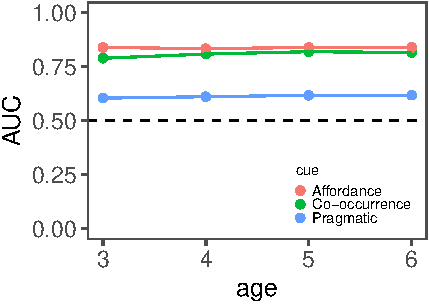
\includegraphics{cogsci_files/figure-latex/dev-1} 

}

\caption{\label{fig:dev} The Area Under the ROC Curve (AUC) scores for each cue (across all categories) using speech heard by children up to a particular age. A value of 0.5 represents pure chance, and a value of 1 represents perfect performance.}\label{fig:dev}
\end{figure}
\end{CodeChunk}

\hypertarget{general-discussion}{%
\section{General Discussion}\label{general-discussion}}

How do children acquire the complex hierarchical relationships that
characterize mature human conceptual knowledge? In both its explicit
statements and implicit distributional structure, caregiver talk
provides a rich source of information about conceptual relationships.
Here we used a distributional approach to compare the relative
importance of different information sources in categorization of six
common superordinate categories. We found that distributional
information (as captured by Word2Vec models) and verb affordances were
effective and that -- to a lesser extent -- sentential co-occurrence
with superordinate labels also contributed positively to classification.
Thus, at a high level, our study confirms the utility of caregiver talk
for conveying conceptual information and suggests that a rich range of
linguistic cues may be available to children in learning category
structure.

This work takes a first step towards integrating different conceptual
information sources from caregiver language, but it has a number of
limitations that should be addressed in future work. First, we conducted
our study in English with the data available in CHILDES, but
cross-linguistic and cross-cultural work is necessary to understand
variation in the way that caregivers' language specifies the categorical
structure of the world (Medin, Bennis, \& Chandler, 2010). Second, we
used rough approximations of the potentially more subtle cues that we
labeled ``pragmatic'' and ``verb affordance'' information. Capturing the
structure of knowledge as it is used in natural language is an open
computational challenge, but we could likely improve performance
substantially by further refining these cues.

Our work here suggests the presence of multiple information sources
about conceptual structure in children's linguistic environment. Perhaps
the most exciting future direction is the development of cognitive
models that make use of this information in a principled way, and that
synthesize it with knowledge gleaned from other modalities including
children's direct observations of the world around them. Such a
synthesis will be crucial in making progress on understanding children's
conceptual structure. By refining our understanding of linguistic cues
to conceptual hierarchy, we hope our work here helps take a first step
in this broader project.

\hypertarget{references}{%
\section{References}\label{references}}

\setlength{\parindent}{-0.1in} 
\setlength{\leftskip}{0.125in}

\noindent

\hypertarget{refs}{}
\leavevmode\hypertarget{ref-blewitt1983}{}%
Blewitt, P. (1983). Dog versus collie: Vocabulary in speech to young
children. \emph{Developmental Psychology}, \emph{19}(4).

\leavevmode\hypertarget{ref-callanan1985}{}%
Callanan, M. A. (1985). How parents label objects for young children:
The role of input in the acquisition of category hierarchies.
\emph{Child Development}, 508--523.

\leavevmode\hypertarget{ref-callanan1989}{}%
Callanan, M. A. (1989). Development of object categories and inclusion
relations: Preschoolers' hypotheses about word meanings.
\emph{Developmental Psychology}, \emph{25}(2).

\leavevmode\hypertarget{ref-carey1987}{}%
Carey, S. (1987). \emph{Conceptual change in childhood}. MIT Press.

\leavevmode\hypertarget{ref-chi1989}{}%
Chi, M. T., Hutchinson, J. E., \& Robin, A. F. (1989). How inferences
about novel domain-related concepts can be constrained by structured
knowledge. \emph{Merrill-Palmer Quarterly (1982-)}, 27--62.

\leavevmode\hypertarget{ref-clark1997}{}%
Clark, E. V. (1997). Conceptual perspective and lexical choice in
acquisition. \emph{Cognition}, \emph{64}(1), 1--37.

\leavevmode\hypertarget{ref-fenson94}{}%
Fenson, L., Dale, P. S., Reznick, J. S., Bates, E., Thal, D. J.,
Pethick, S. J., \ldots{} Stiles, J. (1994). Variability in early
communicative development. \emph{Monographs of the Society for Research
in Child Development}, \emph{59}(5), i--185.

\leavevmode\hypertarget{ref-fisher2011}{}%
Fisher, A. V., Matlen, B. J., \& Godwin, K. E. (2011). Semantic
similarity of labels and inductive generalization: Taking a second look.
\emph{Cognition}, \emph{118}(3).

\leavevmode\hypertarget{ref-fourtassi2019}{}%
Fourtassi, A., Scheinfeld, I., \& Frank, M. C. (2019). The development
of abstract concepts in children's early lexical networks. In
\emph{Proceedings of the workshop on cognitive modeling and
computational linguistics} (pp. 129--133).

\leavevmode\hypertarget{ref-harris1957}{}%
Harris, Z. S. (1957). Co-occurrence and transformation in linguistic
structure. \emph{Language}, \emph{33}(3).

\leavevmode\hypertarget{ref-huebner2018}{}%
Huebner, P. A., \& Willits, J. A. (2018). Structured semantic knowledge
can emerge automatically from predicting word sequences in
child-directed speech. \emph{Frontiers in Psychology}, \emph{9}, 133.

\leavevmode\hypertarget{ref-inagaki2002}{}%
Inagaki, K., \& Hatano, Giyoo. (2002). \emph{Young children's naive
thinking about the biological world}. New York : Psychology Press.

\leavevmode\hypertarget{ref-inhelder2013}{}%
Inhelder, B., \& Piaget, J. (2013). \emph{The early growth of logic in
the child: Classification and seriation}. Routledge.

\leavevmode\hypertarget{ref-keil1981}{}%
Keil, F. C. (1981). Constraints on knowledge and cognitive development.
\emph{Psychological Review}, \emph{88}(3).

\leavevmode\hypertarget{ref-landauer1997}{}%
Landauer, T. K., \& Dumais, S. T. (1997). A solution to plato's problem:
The latent semantic analysis theory of acquisition, induction, and
representation of knowledge. \emph{Psychological Review}, \emph{104}(2).

\leavevmode\hypertarget{ref-liu2001}{}%
Liu, J., Golinkoff, R. M., \& Sak, K. (2001). One cow does not an animal
make: Young children can extend novel words at the superordinate level.
\emph{Child Development}, \emph{72}(6), 1674--1694.

\leavevmode\hypertarget{ref-macwhinney2014}{}%
MacWhinney, B. (2014). \emph{The childes project: Tools for analyzing
talk, volume ii: The database}. Psychology Press.

\leavevmode\hypertarget{ref-matlen2015}{}%
Matlen, B. J., Fisher, A. V., \& Godwin, K. E. (2015). The influence of
label co-occurrence and semantic similarity on children's inductive
generalization. \emph{Frontiers in Psychology}, \emph{6}.

\leavevmode\hypertarget{ref-medin2010}{}%
Medin, D., Bennis, W., \& Chandler, M. (2010). Culture and the
home-field disadvantage. \emph{Perspectives on Psychological Science},
\emph{5}(6).

\leavevmode\hypertarget{ref-mikolov2013}{}%
Mikolov, T., Sutskever, I., Chen, K., Corrado, G. S., \& Dean, J.
(2013). Distributed representations of words and phrases and their
compositionality. In \emph{Advances in neural information processing
systems} (pp. 3111--3119).

\leavevmode\hypertarget{ref-saffran1996}{}%
Saffran, J. R., Aslin, R. N., \& Newport, E. L. (1996). Statistical
learning by 8-month-old infants. \emph{Science}, \emph{274}(5294),
1926--1928.

\leavevmode\hypertarget{ref-sanchez2019}{}%
Sanchez, A., Meylan, S. C., Braginsky, M., MacDonald, K. E., Yurovsky,
D., \& Frank, M. C. (2019). Childes-db: A flexible and reproducible
interface to the child language data exchange system. \emph{Behavior
Research Methods}, \emph{51}(4), 1928--1941.

\leavevmode\hypertarget{ref-shipley1983}{}%
Shipley, E. F., Kuhn, I. F., \& Madden, E. C. (1983). Mothers' use of
superordinate category terms. \emph{Journal of Child Language},
\emph{10}(3).

\leavevmode\hypertarget{ref-sloutsky2015}{}%
Sloutsky, V. (2015). Conceptual development. \emph{Handbook of Child
Psychology and Developmental Science}, 1--50.

\bibliographystyle{apacite}


\end{document}
